\documentclass[tikz]{standalone}
\usepackage{tikz}
\usetikzlibrary{positioning}
\usetikzlibrary{calc}

\begin{document}

% Use A4 portrait page, content rotated
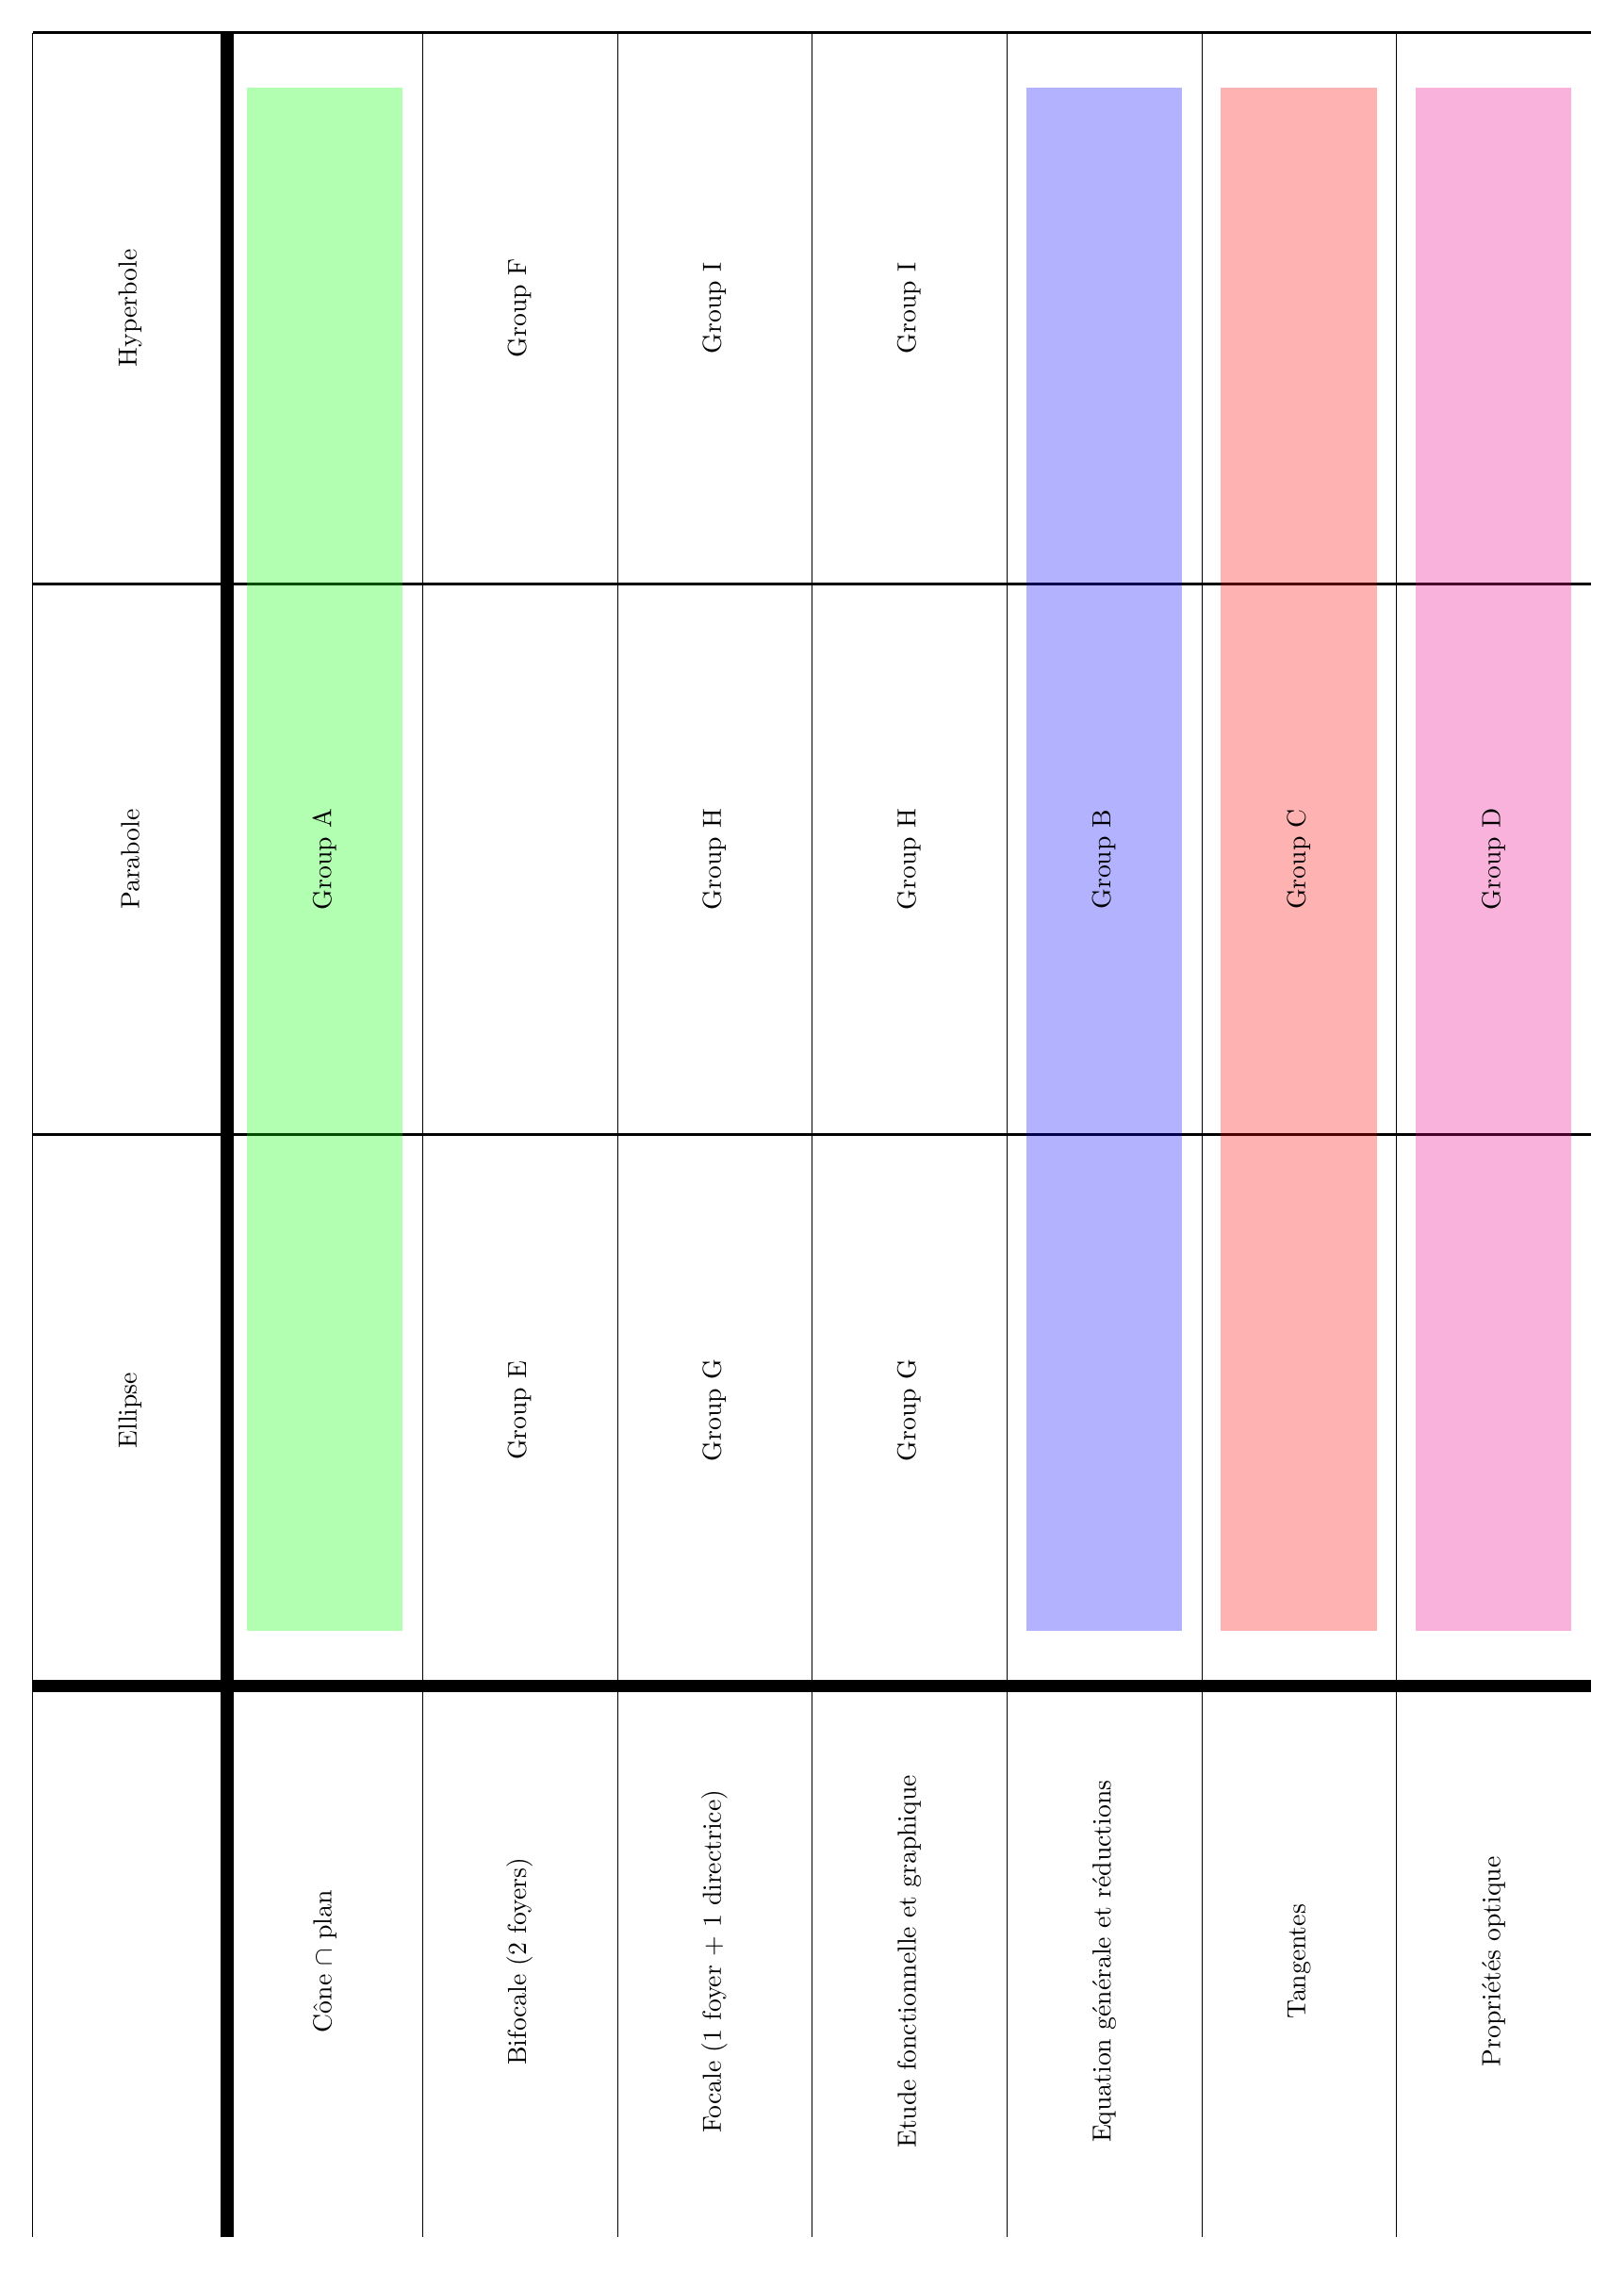
\begin{tikzpicture}[x=1cm, y=1cm]

% Rotate entire content (including text)
\begin{scope}[rotate=90, shift={(0,-21)}] % 21 = A4 height in cm

% Grid size
\def\rows{8}
\def\cols{4}
\def\rowsmin{7}

\def\pagewidth{29.7}
\def\pageheight{21}

\pgfmathsetmacro{\cellwidth}{\pagewidth/\cols}
\pgfmathsetmacro{\cellheight}{\pageheight/\rows}

%colonne
\draw[line width = 5pt] (\cellwidth,0) -- (\cellwidth,\pageheight);

%ligne
\draw[line width = 5pt] (0,\rowsmin*\cellheight) -- (\pagewidth,\rowsmin*\cellheight);

% Draw grid
\foreach \i in {2,...,\cols} {
    \draw[line width = 1pt] (\i*\cellwidth,0) -- (\i*\cellwidth,\pageheight);
}
\foreach \j in {1,...,\rows} {
    \draw[line width = 0.1pt] (0,\j*\cellheight) -- (\pagewidth,\j*\cellheight);
}

% Draw rectangles with rotated text

\node[rotate=90] at ($ (0,\rowsmin*\cellheight) + (1.5*\cellwidth,0.5*\cellheight) $) {Ellipse};
\node[rotate=90] at ($ (0,\rowsmin*\cellheight) + (2.5*\cellwidth,0.5*\cellheight) $) {Parabole};
\node[rotate=90] at ($ (0,\rowsmin*\cellheight) + (3.5*\cellwidth,0.5*\cellheight) $)  {Hyperbole};

\node[rotate=90] at ($ (0,\rowsmin*\cellheight) + (0.5*\cellwidth,-0.5*\cellheight) $) {Cône $\cap$ plan};
\node[rotate=90] at ($ (0,\rowsmin*\cellheight) + (0.5*\cellwidth,-1.5*\cellheight) $) {Bifocale (2 foyers)};
\node[rotate=90] at ($ (0,\rowsmin*\cellheight) + (0.5*\cellwidth,-2.5*\cellheight) $) {Focale (1 foyer + 1 directrice)};
\node[rotate=90] at ($ (0,\rowsmin*\cellheight) + (0.5*\cellwidth,-3.5*\cellheight) $) {Etude fonctionnelle et graphique};
\node[rotate=90] at ($ (0,\rowsmin*\cellheight) + (0.5*\cellwidth,-4.5*\cellheight) $) {Equation générale et réductions};
\node[rotate=90] at ($ (0,\rowsmin*\cellheight) + (0.5*\cellwidth,-5.5*\cellheight) $) {Tangentes};
\node[rotate=90] at ($ (0,\rowsmin*\cellheight) + (0.5*\cellwidth,-6.5*\cellheight) $) {Propriétés optique};





\fill[green,opacity=0.3] (1.1*\cellwidth,6.1*\cellheight) rectangle (3.9*\cellwidth,6.9*\cellheight);
\node[rotate=90] at (2.5*\cellwidth,6.5*\cellheight) {Group A};




\fill[blue,opacity=0.3] (1.1*\cellwidth,2.1*\cellheight) rectangle (3.9*\cellwidth,2.9*\cellheight);
\node[rotate=90] at (2.5*\cellwidth,2.5*\cellheight) {Group B};

\fill[red,opacity=0.3] (1.1*\cellwidth,1.1*\cellheight) rectangle (3.9*\cellwidth,1.9*\cellheight);
\node[rotate=90] at (2.5*\cellwidth,1.5*\cellheight) {Group C};
\fill[magenta,opacity=0.3] (1.1*\cellwidth,0.1*\cellheight) rectangle (3.9*\cellwidth,0.9*\cellheight);
\node[rotate=90] at (2.5*\cellwidth,0.5*\cellheight) {Group D};


\node[rotate=90] at (1.5*\cellwidth,5.5*\cellheight) {Group E};
\node[rotate=90] at (3.5*\cellwidth,5.5*\cellheight) {Group F};
\node[rotate=90] at (1.5*\cellwidth,4.5*\cellheight) {Group G};
\node[rotate=90] at (2.5*\cellwidth,4.5*\cellheight) {Group H};
\node[rotate=90] at (3.5*\cellwidth,4.5*\cellheight) {Group I};
\node[rotate=90] at (1.5*\cellwidth,3.5*\cellheight) {Group G};
\node[rotate=90] at (2.5*\cellwidth,3.5*\cellheight) {Group H};
\node[rotate=90] at (3.5*\cellwidth,3.5*\cellheight) {Group I};
\end{scope}

\end{tikzpicture}

\end{document}